%%%%%%%%%%%%%%%%%%%%%%%%%%%%%%%%%%%%%%%%%%%%%%%%%%%%%%%%
%%%%%%%%%------RMIT SPACE POSTER------------%%%%%%%%%%%%
%%%%%%%%%%%%%%%%%%%%%%%%%%%%%%%%%%%%%%%%%%%%%%%%%%%%%%%%
%%%%%%%%%%%%%%%%%%%%%%%%%%%%%%%%%%%%%%%%%%%%%%%%%%%%%%%%
% a0poster Portrait Poster
%
% The a0poster class was created by:
% Gerlinde Kettl and Matthias Weiser (tex@kettl.de)
% 
% License:
% CC BY-NC-SA 3.0 (http://creativecommons.org/licenses/by-nc-sa/3.0/)
%
% Author/Designer: Timothy Kodikara
%
%% Note: CRC and SERC logos are included in the /figures folder if you might want to use them.
%%%%%%%%%%%%%%%%%%%%%%%%%%%%%%%%%%%%%%%%%
%----------------------------------------------------------------------------------------
%	PACKAGES AND OTHER DOCUMENT CONFIGURATIONS
%----------------------------------------------------------------------------------------
\documentclass[a0,portrait]{a0poster}
%%
\usepackage[top=5cm, bottom=0.3cm, left=5cm, right=3cm]{geometry}
\usepackage[compact]{titlesec}
\usepackage{multicol} % This is so we can have multiple columns of text side-by-side
\columnsep=100pt % This is the amount of white space between the columns in the poster
\columnseprule=15pt % This is the thickness of the blue line between the columns in the poster
\usepackage[svgnames]{xcolor} % Specify colors by their 'svgnames', for a full list of all colors available see here: http://www.latextemplates.com/svgnames-colors
%\usepackage{times} % Use the times font
\usepackage{palatino} % Uncomment to use the Palatino font
\usepackage{xkeyval}
\usepackage{graphicx} % Required for including images
\setlength{\abovecaptionskip}{5pt plus 5pt minus 3pt}
\graphicspath{{figures/}} % Location of the graphics files
\usepackage{booktabs} % Top and bottom rules for table
\usepackage[font=small,labelfont=bf]{caption} % Required for specifying captions to tables and figures
\usepackage{amsfonts, amsmath, amsthm, amssymb} % For math fonts, symbols and environments
\usepackage{csquotes}
\usepackage{wrapfig} % Allows wrapping text around tables and figures
%\usepackage[pdftex]{color}
\def\columnseprulecolor{\color{NavyBlue}}%
\usepackage{framed}
\colorlet{frameborder}{NavyBlue}

%----------------------------------------------------------------------------------------
%	POSTER HEADER 
%----------------------------------------------------------------------------------------
% The header is divided into three boxes:
% The widths of these boxes can be easily edited to accommodate your content as you see fit
\begin{document}
%\hspace*{0.2cm}
\begin{minipage}[c]{\linewidth}
\vspace{0.1cm}
\noindent\makebox[\textwidth][c]{
\begin{minipage}[c]{0.15\linewidth}
\vspace{0pt}\raggedright
\hspace{1cm}

\includegraphics[width=\linewidth]{figures/EPFL-Logo}
\end{minipage}
\hfill
\begin{minipage}[c]{0.70\textwidth}
\centering
\Huge \color{NavyBlue} \textbf{Unsupervised extraction of students navigation patterns on an EPFL MOOC}\\[0.5cm]
\large \color{Black} \textbf{Thibault Asselborn$^{1}$, Victor Faramond$^{1}$, Louis Faucon$^{1}$}\\[0.2cm] % Author(s)
\small 1. \'Ecole Polytechinque F\'ed\'erale de Lausanne, Switzerland\\[0.1cm] % University
\small \texttt{Correspondence: firstname.lastname@epfl.ch}\\
\end{minipage}
%\hfill
\begin{minipage}[c]{0.15\textwidth}
\vspace{0pt}\raggedleft
\hspace{1cm}

\includegraphics[width=0.8\linewidth]{figures/qrcode}
\end{minipage}}
\\[0.1cm]%
% A bit of extra whitespace between the header and poster content
%----------------------------------------------------------------------------------------
\color{NavyBlue}\setlength\FrameRule{25pt}
\begin{framed}
\vspace{0.2cm}
\begin{multicols}{2} % This is how many columns your poster will be broken into, a portrait poster is generally split into 2 columns
%----------------------------------------------------------------------------------------
%	INTRODUCTION
%----------------------------------------------------------------------------------------
\color{Black}
\section*{Introduction}
How do students learn in MOOCs? This project aims at answering this question by analyzing the activities of thousands of students registered on EPFL Scala\footnote{https://www.scala-lang.org/} MOOC hosted by Coursera\footnote{https://www.coursera.org/}. With the rapid growth of MOOCs, Education Science has entered the Big Data bubble, bringing new opportunities to study and improve learning technologies. We are interested in studying students navigation patterns which are the short sequences of learning activities that a students perform on the MOOC platform. In our case, the learning activities are one of watching a video lecture, reading or posting on the forum and submitting assignments. In this project we use unsupervised machine learning techniques to extract the main navigation patterns of students and gain insights on their behavior. We produce a simple and efficient visualization tool in order to provide feedback to teachers to help them understand the potential difficulties encountered by their students during the course and, if necessary, take actions accordingly.

%----------------------------------------------------------------------------------------
%	Data processing Pipaline
%----------------------------------------------------------------------------------------
\section*{Data processing Pipeline}

\textbf{Data} \\
Our dataset contains the logs describing student's interaction events with the MOOC platform. The events are of three type: \verb|Forum|, \verb|Video| and \verb|Assignment|. Detailed information about the data is displayed in table \ref{tab:logs}

\vspace{0.5cm}
\begin{center}
\begin{tabular}{|l|l|l|}
  \hline
  \verb|Forum| & \verb|Video| & \verb|Assignment| \\
  \hline
  \verb|StudentID| & \verb|StudentID| & \verb|StudentID| \\ 
  \verb|Timestamp| & \verb|Timestamp| & \verb|Timestamp| \\
  \verb|EventSubType| & \verb|EventSubType| & \verb|EventSubType| \\
  & \verb|OpenTime| & \verb|OpenTime| \\
  & \verb|VideoID| & \verb|ProblemID| \\
  & & \verb|Grade| \\
  & & \verb|HardCloseTime| \\
  \hline
\end{tabular}
\captionof{table}{Schema of log data from the MOOC}
\label{tab:logs}
\end{center}
\vspace{0.5cm}

\textbf{Preprocessing}
\begin{itemize}
\item Remove events before the beginning and after the end of the course
\item Remove the unnecessary data
\item Remove students not working on assignments
\end{itemize}

\textbf{Feature engineering} \\ 
We extract students navigation patterns for each assignment of the course and transform these patterns into vectors of features describing them. Our features are designed to capture the learning behavior of students such as for example \verb|numberOfVideoBeforeFirstProblem| and \verb|numberOfProblemEvent|, describing respectively the number of lectures watched by a student before submitting the assignment and the number of time the student submitted the assignment. The complete set of features is displayed on figure \ref{fig:kmeans}.

\begin{center}
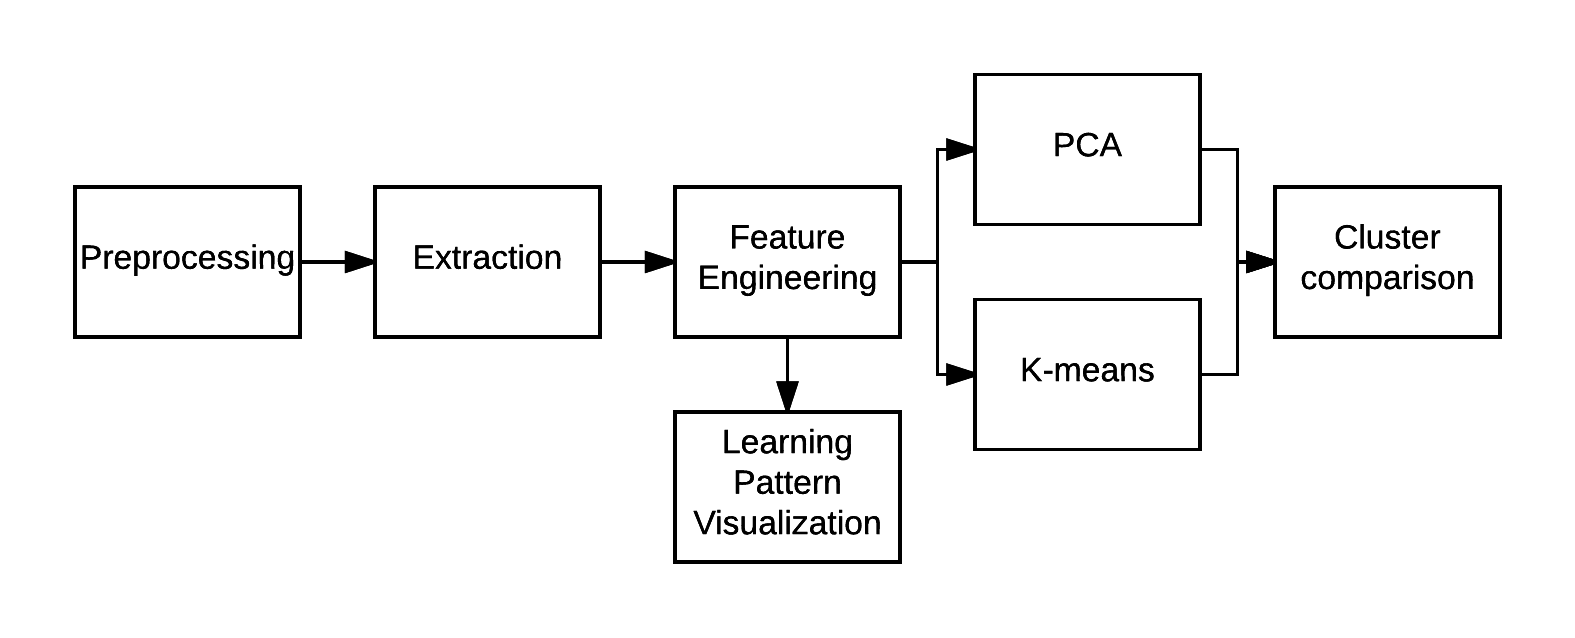
\includegraphics[width=0.4\textwidth]{figures/process}
\end{center}
\captionof{figure}{Processing Pipeline}
\label{fig:pipe}

%----------------------------------------------------------------------------------------
%	Visualizing learning patterns
%---------------------------------------------------------------------------------------- 
\section*{Visualizing Learning Patterns}
To visualize the navigation patterns of students, we use Sankey diagrams\footnote{The diagrams were produced using http://sankey.csaladen.es/}. The figure \ref{fig:navigation} shows two such diagrams for two different assignments of the MOOC. We can see at one sight the proportion of students skipping the videos, if a video is repeated or skipped by many students or if students fail their first attempt at the assignment.

\begin{center}
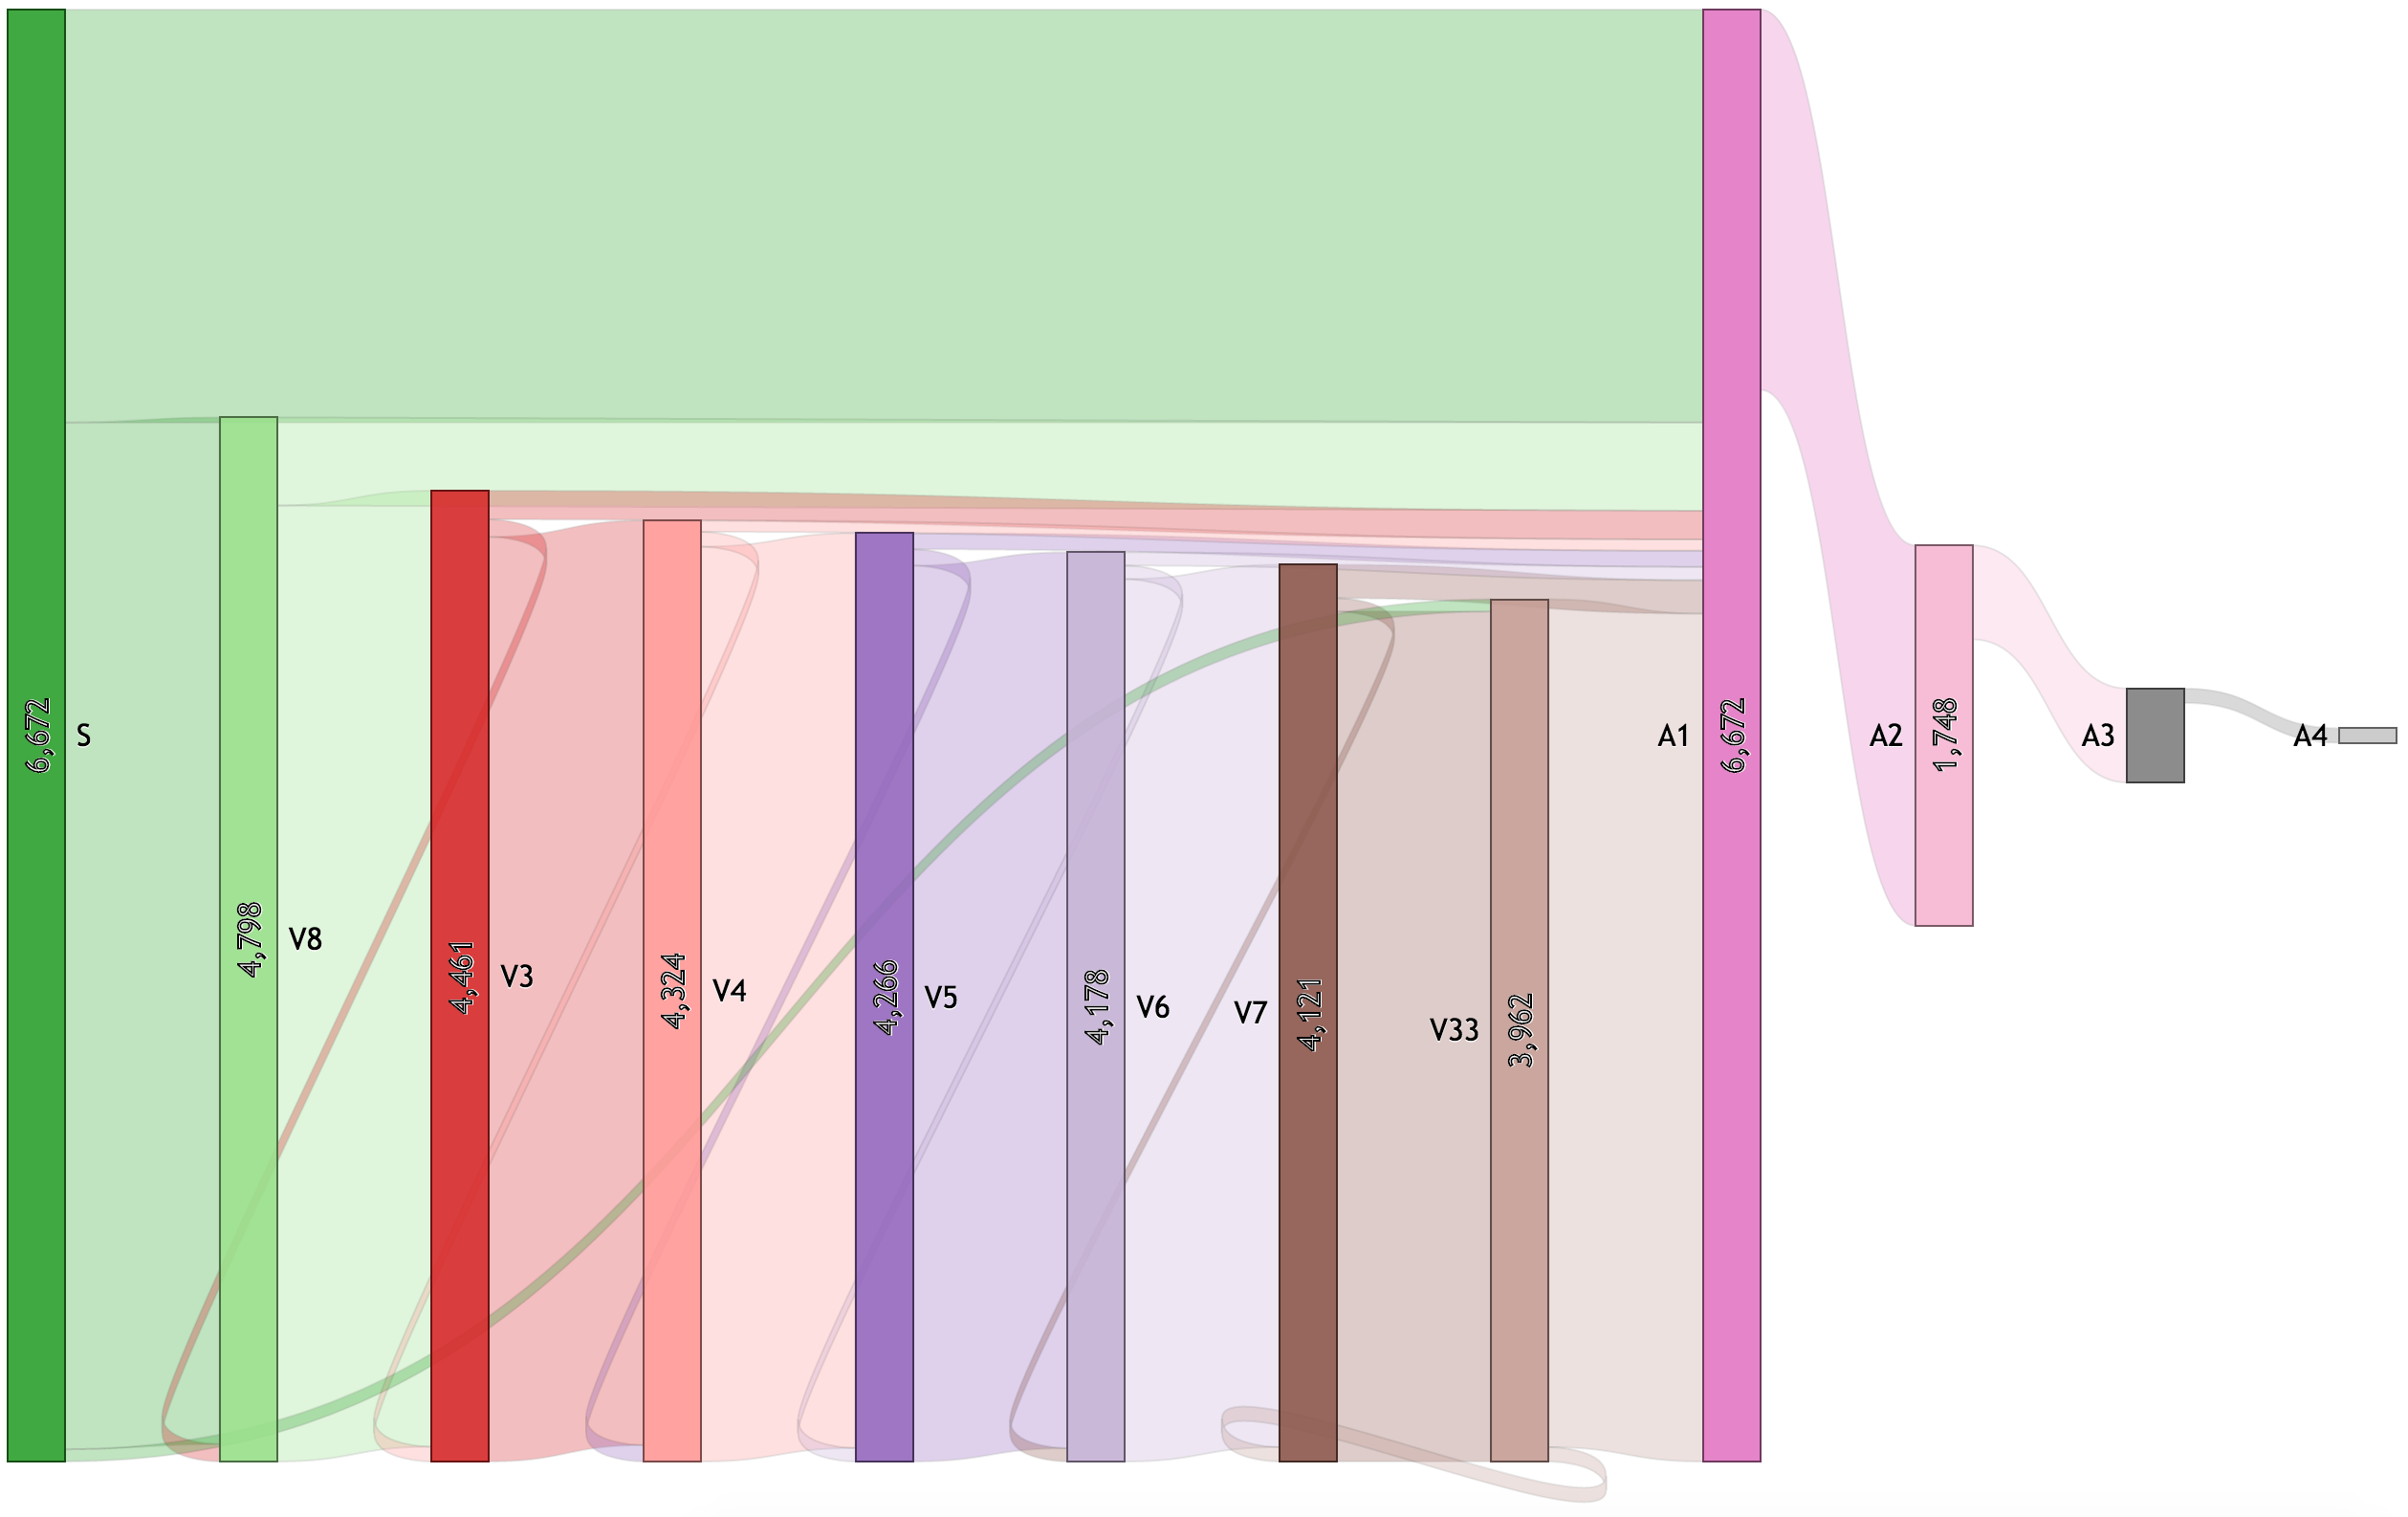
\includegraphics[width=0.23\textwidth]{figures/7}
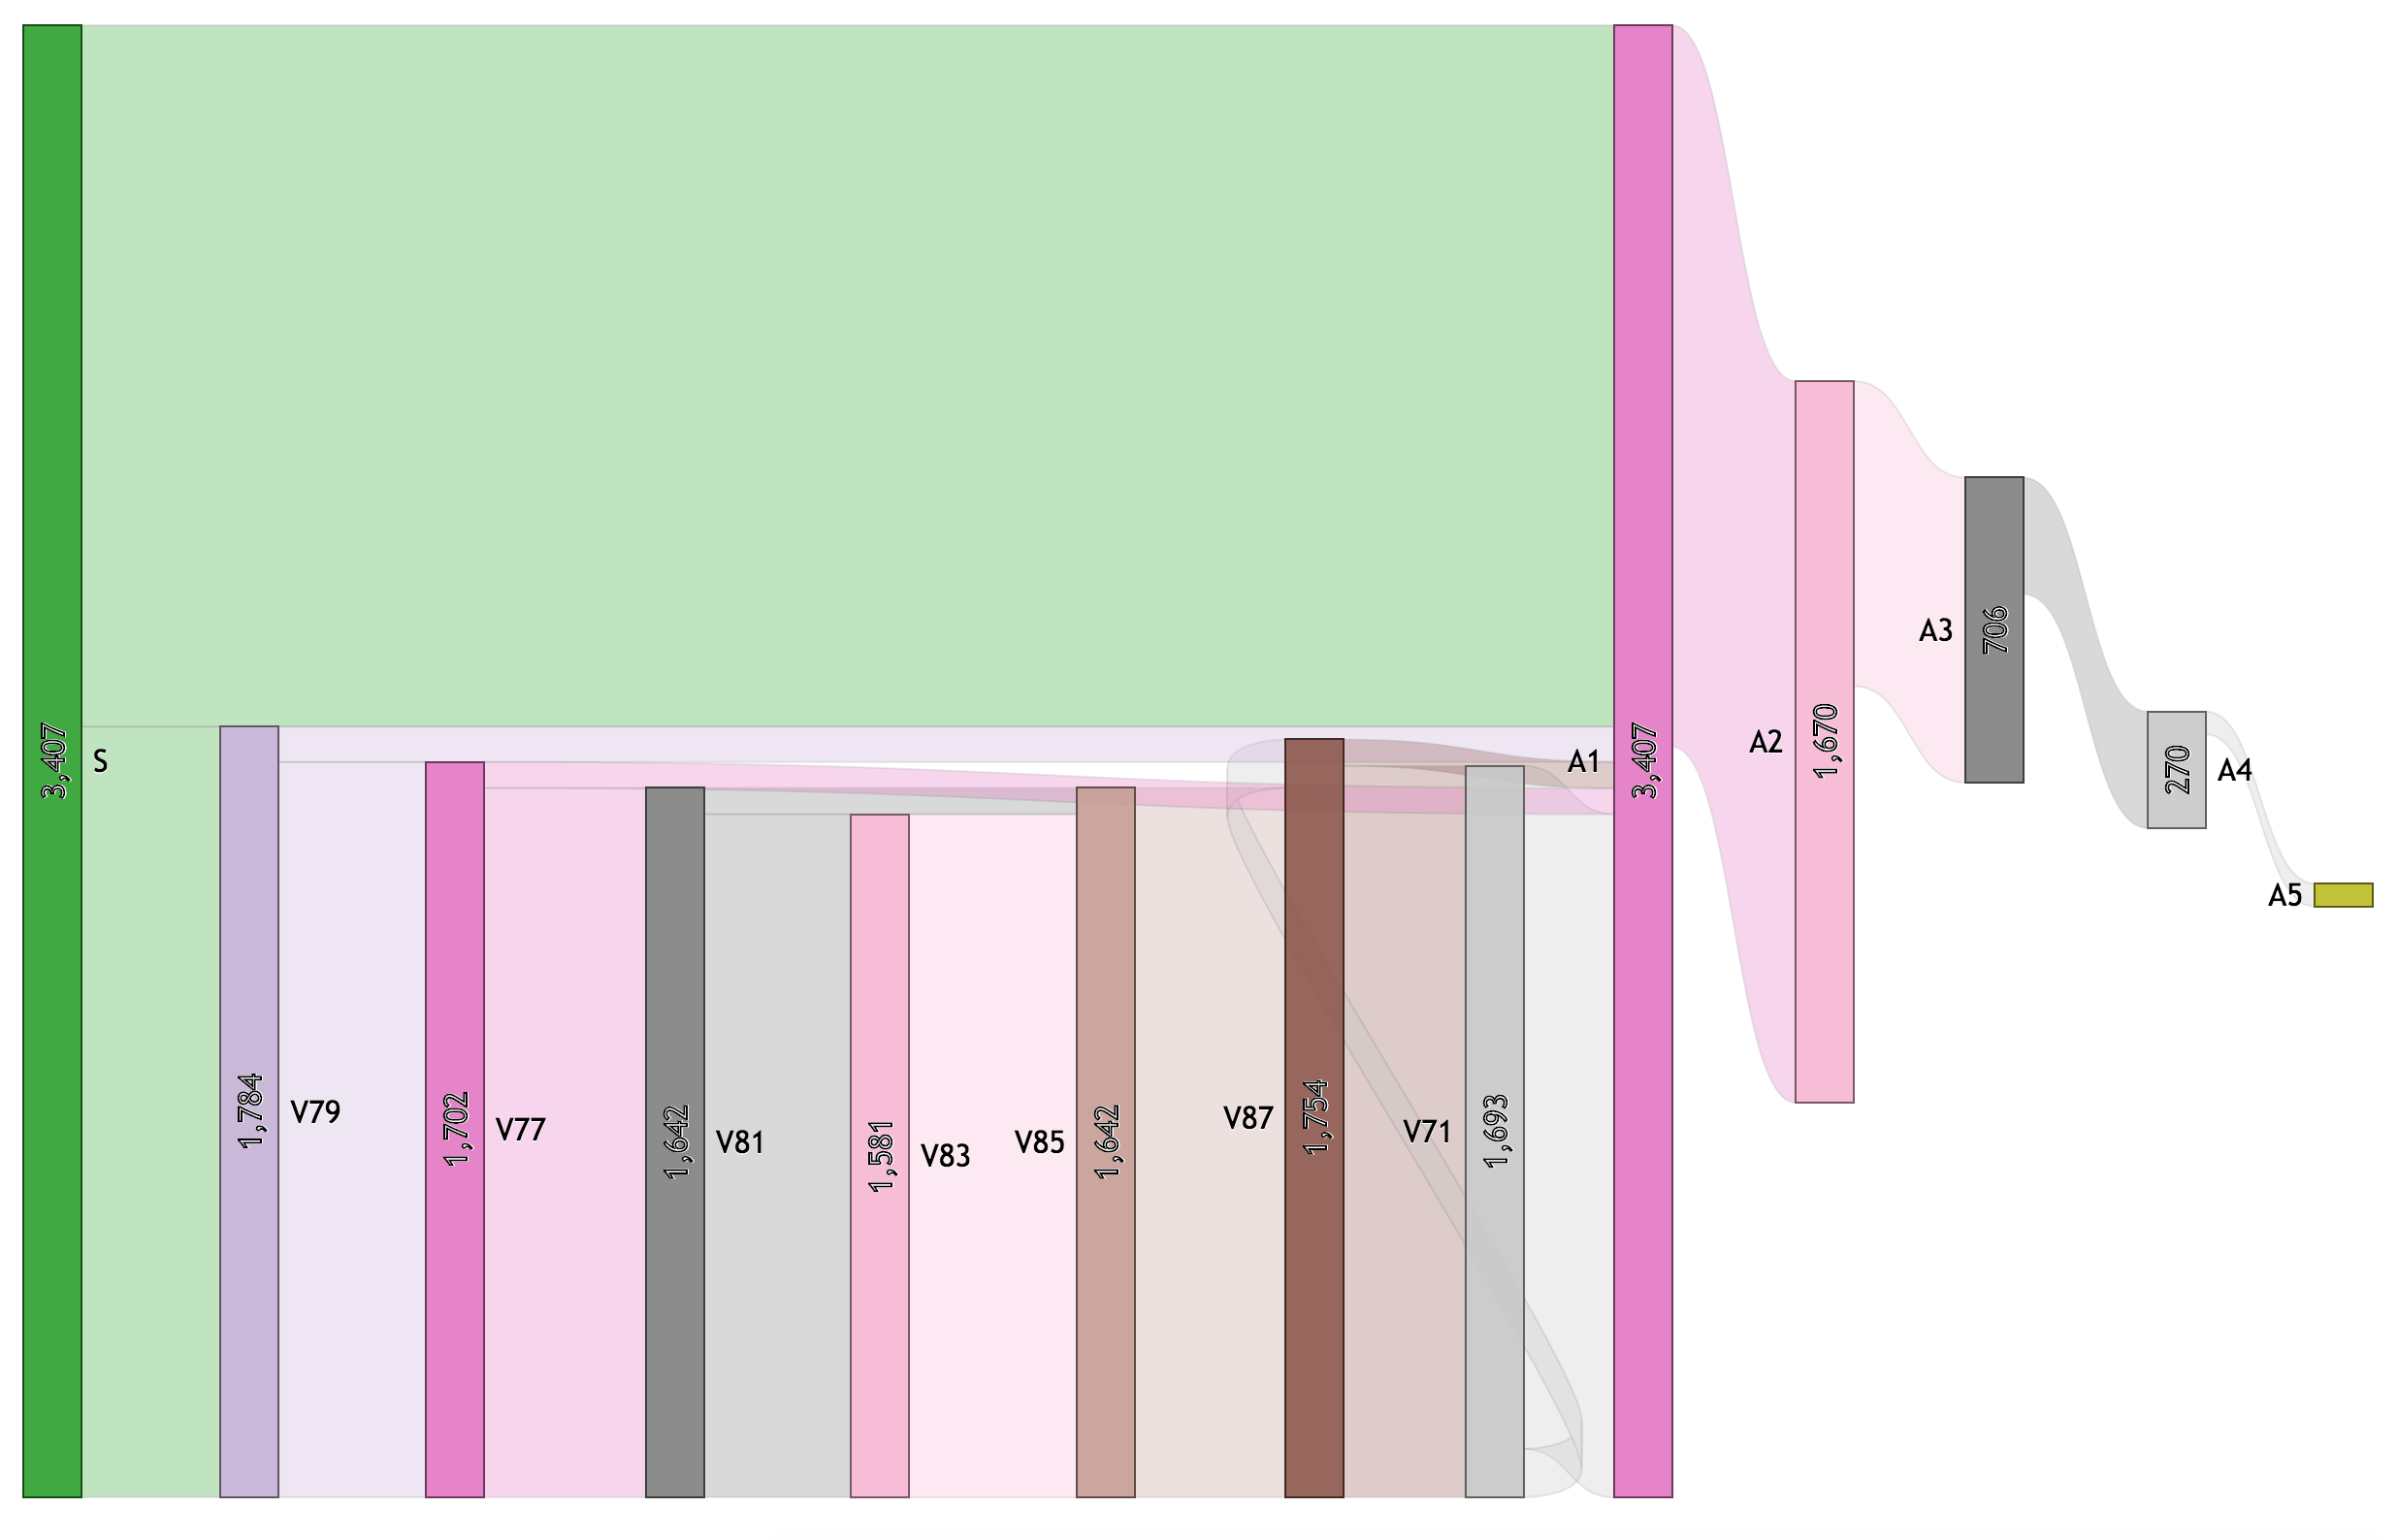
\includegraphics[width=0.23\textwidth]{figures/23}
\end{center}
\captionof{figure}{Navigation patterns of students for two different assignments}
\label{fig:navigation}

%----------------------------------------------------------------------------------------
%	Extracting learning strategies
%---------------------------------------------------------------------------------------- 
\section*{Extracting Clusters of Navigation Patterns}
We apply a K-Means clustering on the navigation patterns' vectors of features, in order to understand the different approaches of students. We chose to divide the patterns into 3 clusters as this separation gave the highest silhouette score. \\

\textbf{Cluster 1}: \textit{Typical students (40.2\% of students)} \\
These patterns high number of videos views. It corresponds to students that spend the longest before working on the assignment. Thus, the lesson seems to be understood as they don't use the video anymore after the first problem submission. It is also the group of students having the best grades.

\textbf{Cluster 2}: \textit{Struggling students (31.3\% of students)} \\
These patterns show students who seem to have some difficulties with the course. It is shown by their first grade lower than the other clusters and also by the higher number of forum events. In this cluster, students submit the problem several times and have to go back to the lesson (lectures are watched after the first attempt).

\textbf{Cluster 3}: \textit{Certificate seekers (28.5\% of students)} \\
These patterns show students who mostly do not watch any videos, do not use the forum and go directly to the problem. They are therefore very fast until submitting their last problem and generally obtain a very good grade. These students seem to already have the knowledge for this course and are show strong motivation in earning the certificate. \\

\begin{center}
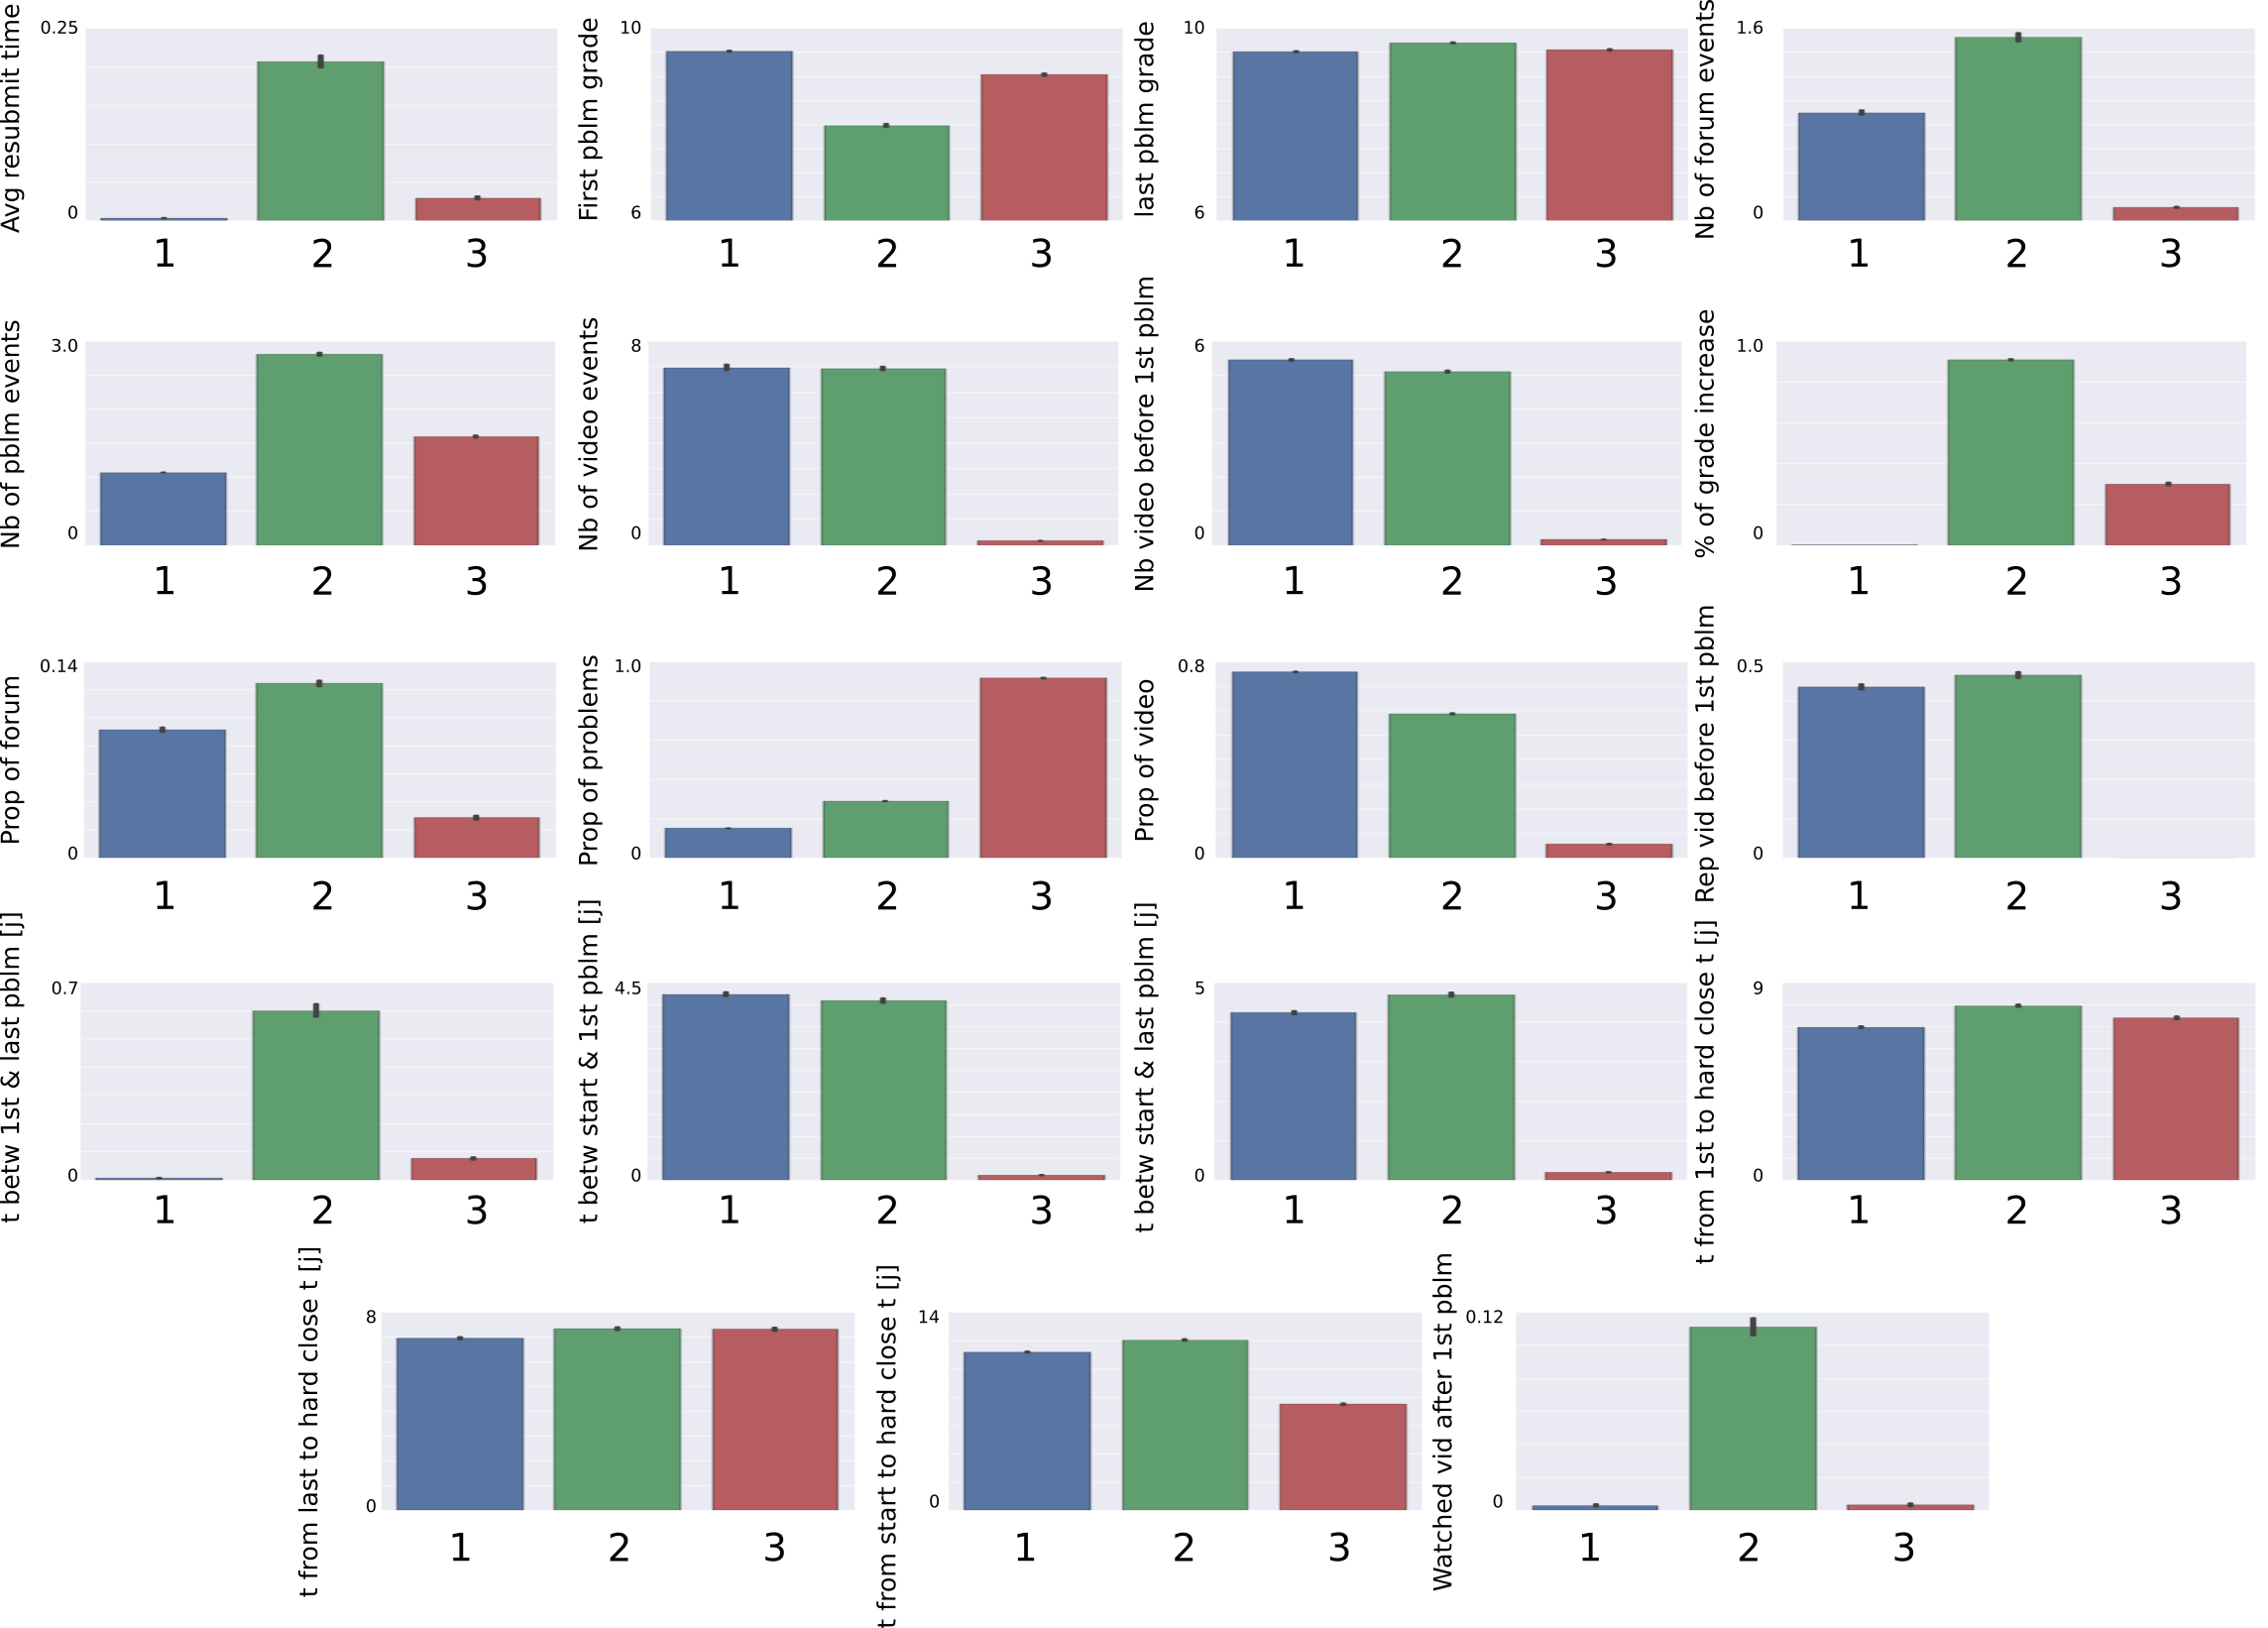
\includegraphics[width=0.95\linewidth]{figures/KMEAN_features}
\captionof{figure}{Average over each feature for the three clusters of navigation patterns extracted with the K-Means algorithm}
\label{fig:kmeans}
\end{center}
\vspace{0.1cm}

\begin{wrapfigure}[23]{R}{0.25\textwidth}
\begin{center}
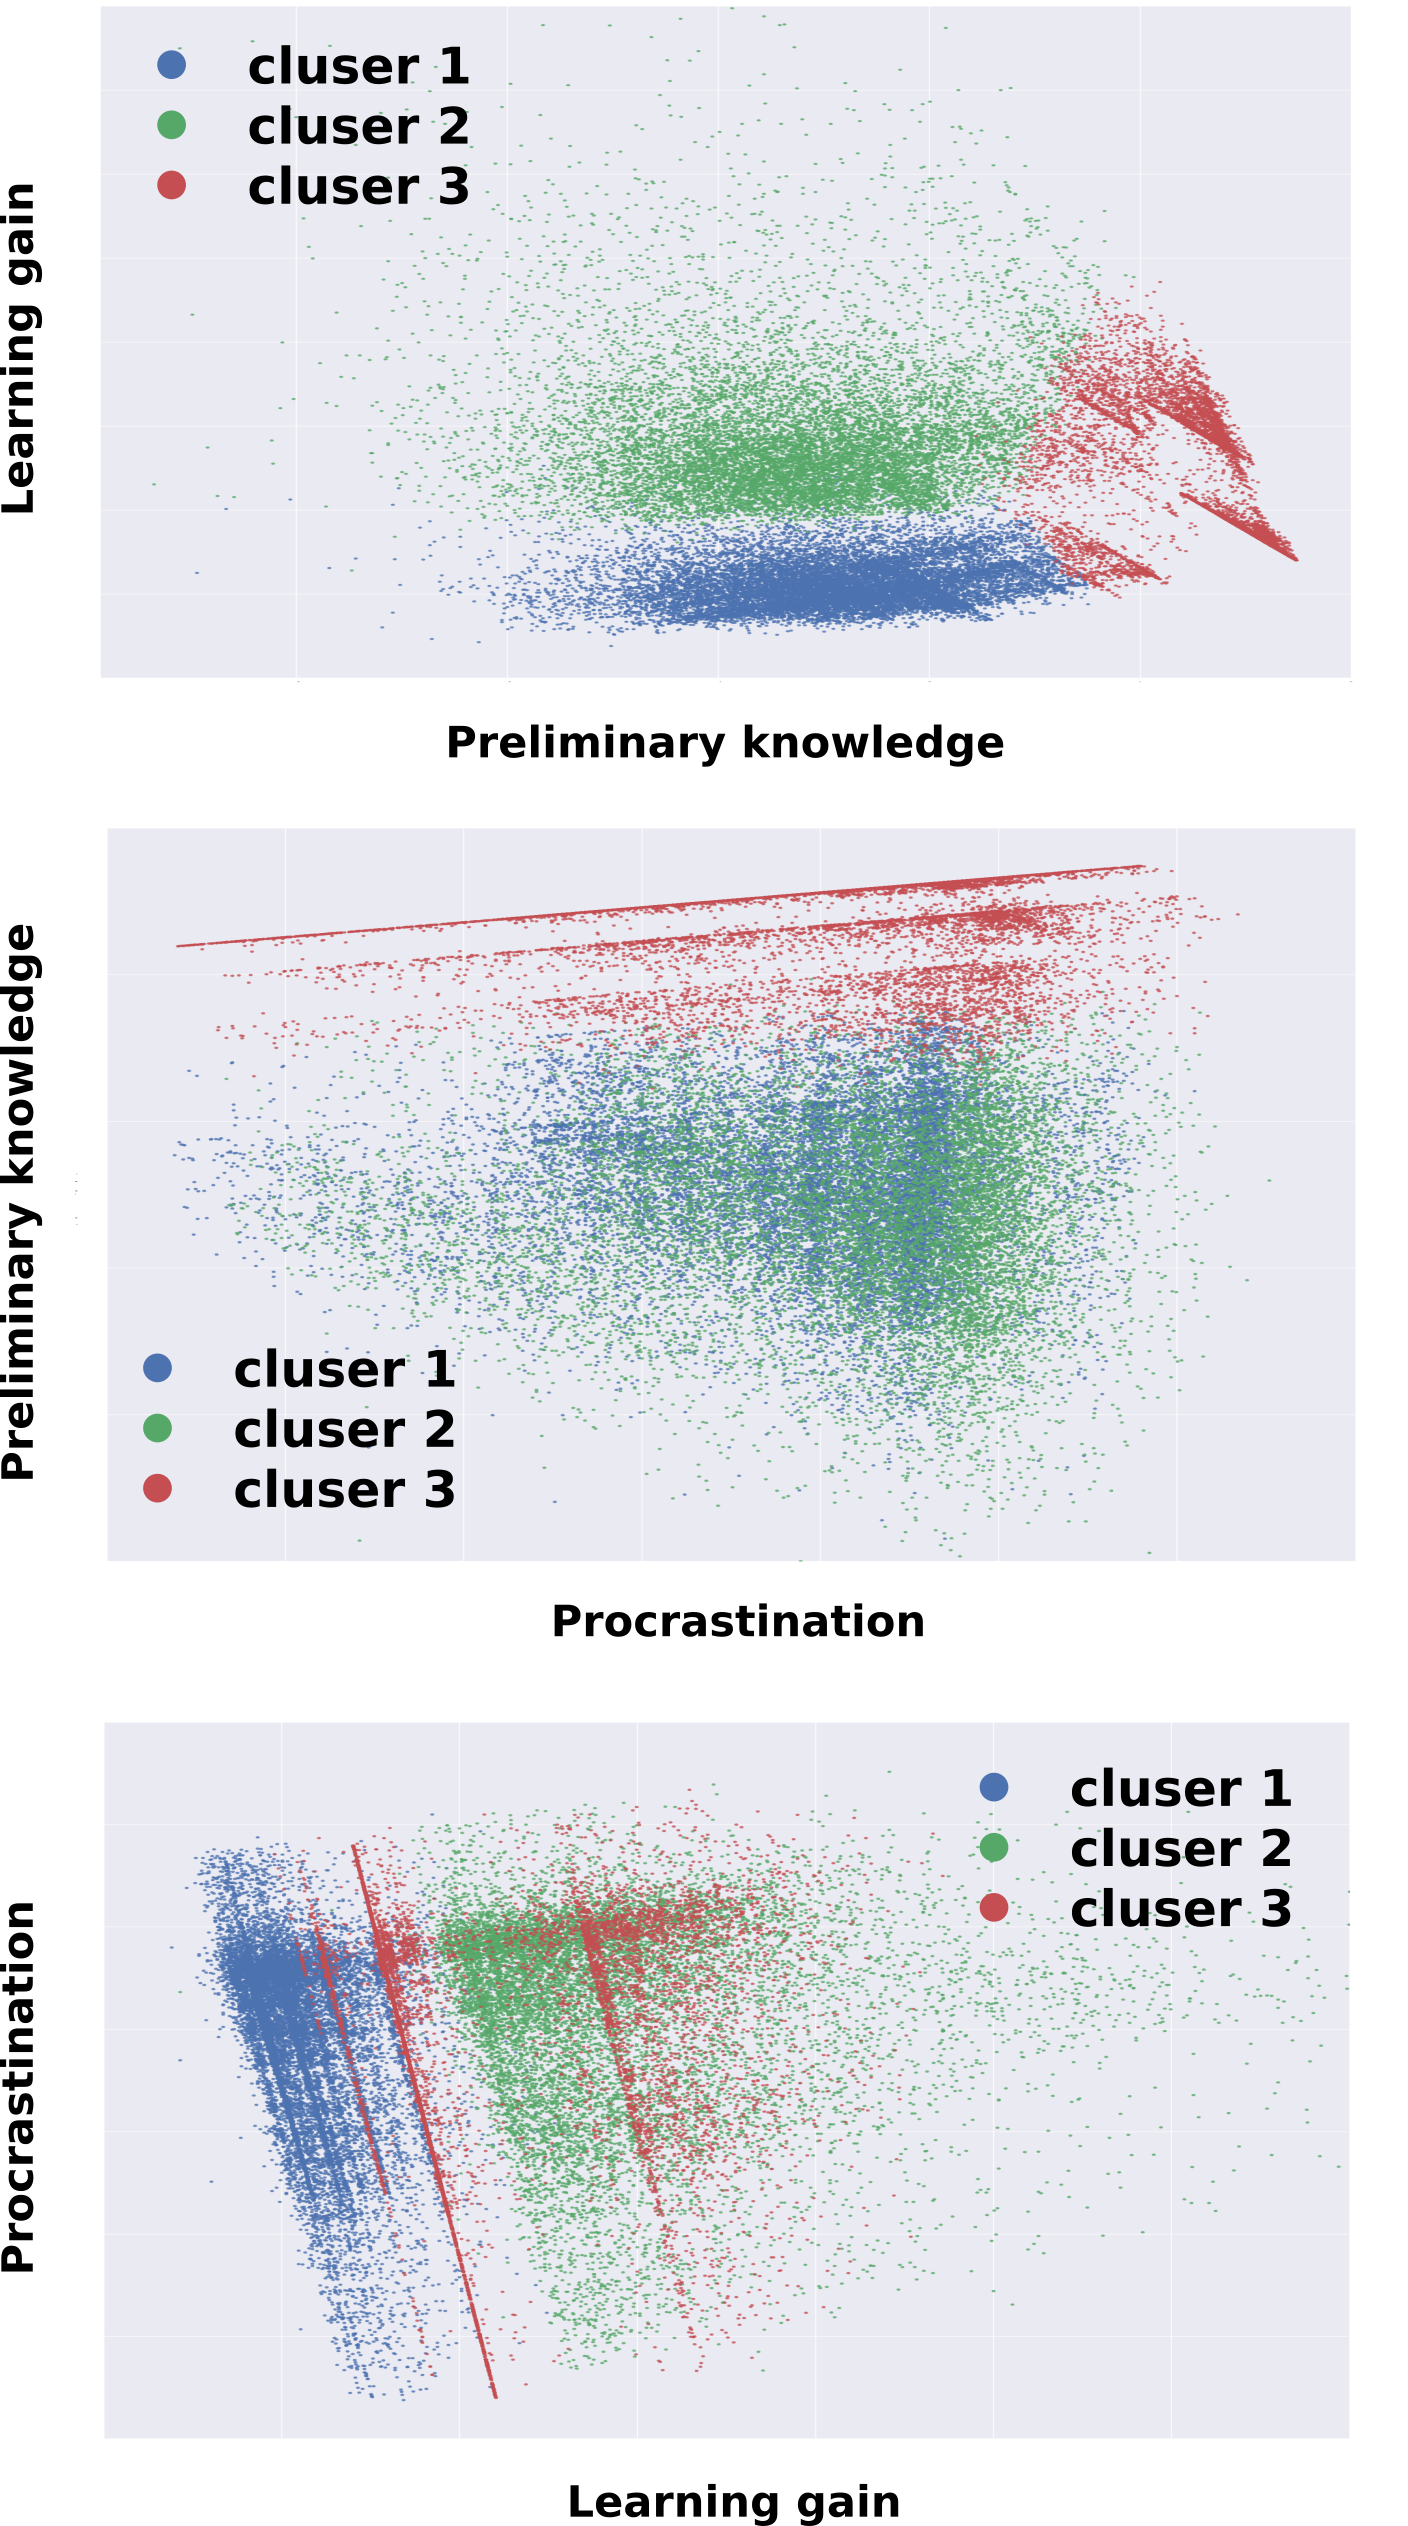
\includegraphics[width=0.2\textwidth]{figures/PCA}
\end{center}
\captionof{figure}{Patterns plotted against the three main principal components.}
\end{wrapfigure}

~\\
We perform a Principal Component Analysis to reveal the main variations between the navigation pattern clusters. \\
\vspace{0.8cm}

\textbf{Component 1} (\textit{25.9\% variance}) \\
\textbf{Preliminary knowledge}: A high value on this component means lesser number of lecture views and higher proportion of problem events.
\vspace{1.5cm}

\textbf{Component 2} (\textit{18.9\% variance}) \\
\textbf{Learning gain}: This component correlates with the increase in grade of students, thus tells us how much they learn.
\vspace{1.5cm}

\textbf{Component 3} (\textit{13.5\% variance}) \\
\textbf{Procrastination}: The navigation patterns with a high value along the third component correspond to shorter time until the assignment deadline.
\vspace{2.25cm}

%----------------------------------------------------------------------------------------
%	Extracting learning strategies
%---------------------------------------------------------------------------------------- 
\section*{Changes of Learning Strategies}
Finally, we provide a visualization of students changes in navigation patterns type along the course. This can show to teachers the proportion of students in each of the three clusters for each assignment. Thus, it can reveal for example an increase in the number of struggling students or a decrease of lecture interest. 

\begin{center}
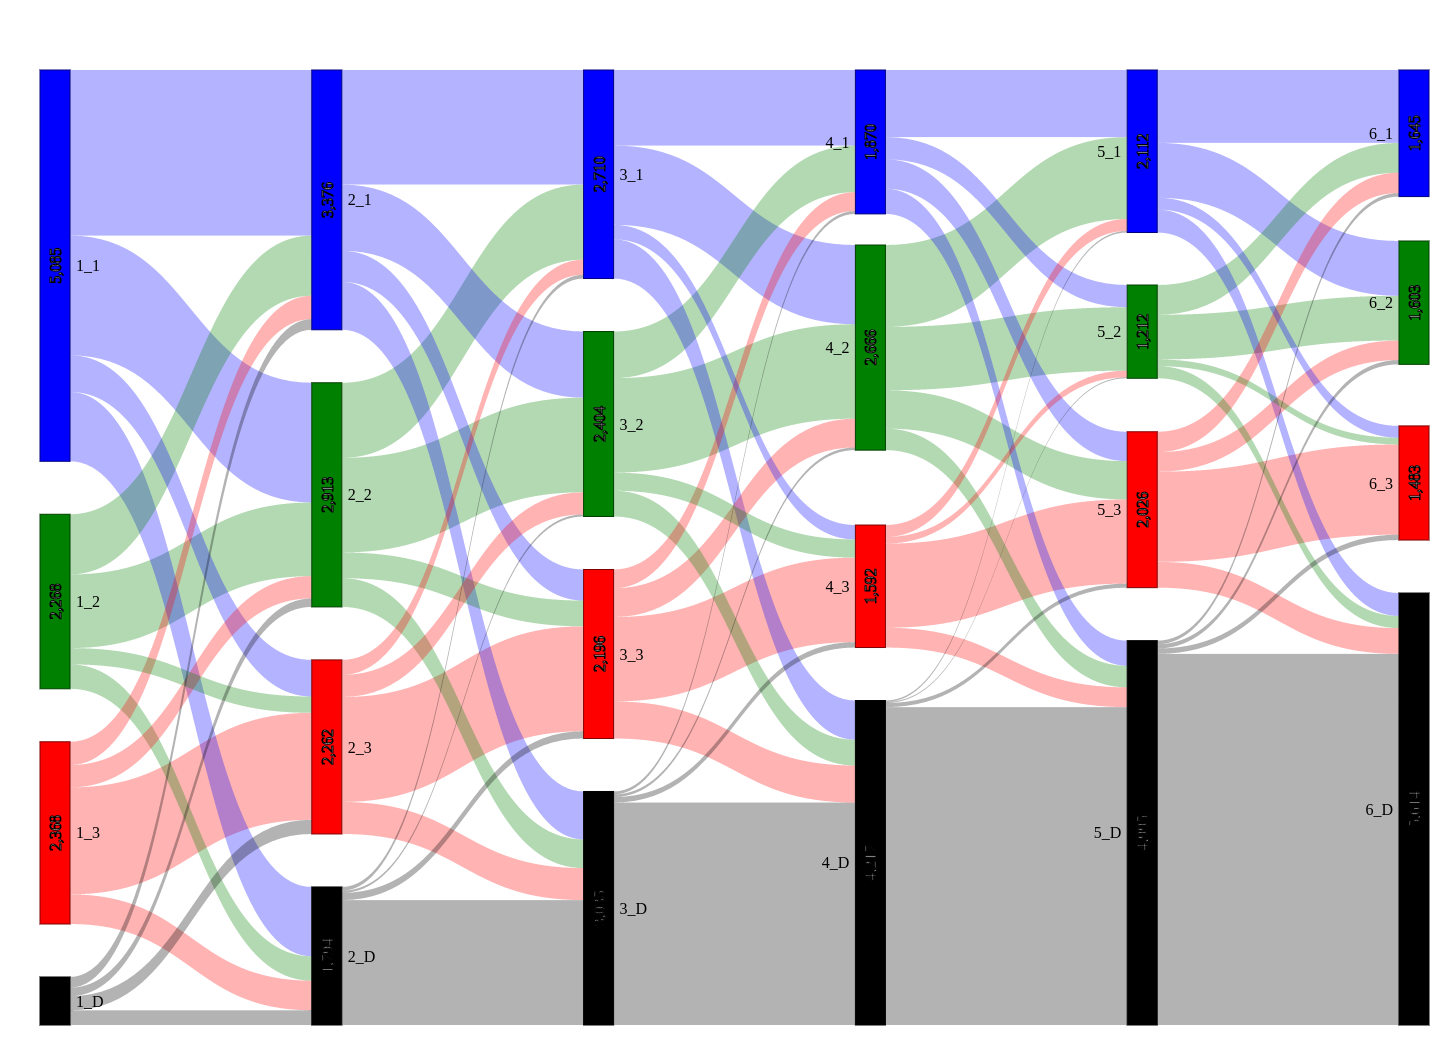
\includegraphics[width=0.4\textwidth]{figures/strategies}
\end{center}
\captionof{figure}{Students choice of learning strategy}
\vspace{0.1cm}

\end{multicols}
%\textcolor{NavyBlue}{\rule{\linewidth}{15pt}}
\vspace{0.5cm}
\end{framed}
\end{minipage}
%\hspace*{0.1cm}
\end{document}
%----------------------------------------------------------------------------------------
%%%%%%%%%%%%%%%%%%%%%%%%%%%%%%%%%%%%%%%%%%%%%%%%%%